\chapter{Additional graphs and analysis}

\section{Sample data from dataset}
\begin{table}[ht]
    \captionsetup{font=small}
    \centering
    \begin{tabularx}{\textwidth}{|l|X|c|c|l|}
        \hline
        \rowcolor[gray]{0.7}
        \textbf{id} & \textbf{text}                                               & \textbf{binarylabel} & \textbf{multilabel} & \textbf{domain} \\
        \hline
        1.20E+17    & asus g60 series . bought it to play games but guess not bf3 & 1                    & 1                   & electronics     \\
        \hline
        4.88E+17    & love this trimmer ! making the sidewalk look sharp <url>    & 0                    & 0                   & other           \\
        \hline
    \end{tabularx}
    \caption{Sample data from \cite{jinModelingSeverityComplaints2021}. The \texttt{binarylabel} represents the label for complaints with 1 indicating the tweet is a complaint. Columns \texttt{id} and \texttt{multilabel} are not used for the experiments}
    \label{tab: apdx_sample_data}
\end{table}

\section{Breakdown of tweets in full dataset}
\begin{table}[ht]
    \captionsetup{font=small}
    \centering
    \begin{tabularx}{\textwidth}{|X|c|c|c|}
        \hline
        \rowcolor[gray]{0.7}
        \textbf{Domains}            & \textbf{Complaints} & \textbf{Non-Complaints} & \textbf{Total Tweets} \\
        \hline
        Food \& Beverage            & 95 \small{(73\%)}   & 35 \small{(27\%)}       & 130 \small{(7\%)}     \\
        \rowcolor[gray]{0.9}
        Apparel                     & 145 \small{(55.3\%)}  & 117 \small{(44.7\%)}      & 258 \small{(13\%)}    \\
        Retail                      & 124 \small{(62\%)}  & 75 \small{(38\%)}       & 199 \small{(10\%)}    \\
        \rowcolor[gray]{0.9}
        Cars                        & 67 \small{(73\%)}   & 25 \small{(27\%)}       & 92 \small{(4\%)}      \\
        Services                    & 207 \small{(61\%)}  & 130 \small{(39\%)}      & 337 \small{(17\%)}    \\
        \rowcolor[gray]{0.9}
        Software \& Online Services & 189 \small{(65\%)}  & 103 \small{(35\%)}      & 292 \small{(15\%)}    \\
        Transport                   & 139 \small{(56\%)}  & 109 \small{(44\%)}      & 248 \small{(12\%)}    \\
        \rowcolor[gray]{0.9}
        Electronics                 & 174 \small{(61\%)}  & 112 \small{(39\%)}      & 286 \small{(15\%)}    \\
        Other                       & 96 \small{(79\%)}   & 33 \small{(21\%)}       & 129 \small{(7\%)}     \\
        \hline
        \rowcolor[gray]{0.9}
        \textbf{Total}              & 1232 \small{(63\%)} & 739 \small{(37\%)}      & 1971                  \\
        \hline
    \end{tabularx}
    \caption{The nine domains and the distribution of tweets that are complaints and those that are not. The percentages indicate how the splits are distributed \cite{preotiuc-pietro_automatically_2019}.}
    \label{tab: domains}
\end{table}


\section{Token distribution after tokenization}
\label{sec: apdxa_token_dist}
The graphs in Figure \ref{fig: apdxa_tokens} show the distribution of token size for tweets from the full dataset for each of the models based on the tokenizer they use. The graph for BERT base uncased is in Chapter 3, Figure \ref{fig: bef_aft_token}.
\begin{figure}[htbp]
    \centering
    \captionsetup{font=small}
    \begin{subfigure}[b]{0.48\textwidth}
        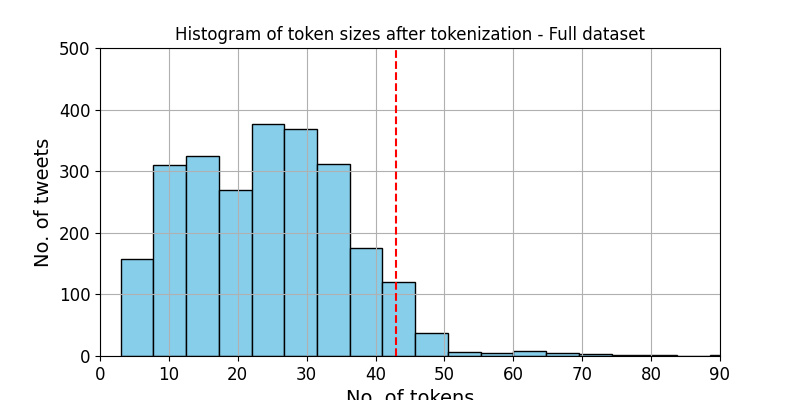
\includegraphics[width=\textwidth]{figures/token_pp_hist_albert-base-v2.png}
        \caption{Albert base}
        \label{fig: token_pp_hist_albert}
    \end{subfigure}
    \hfill
    \begin{subfigure}[b]{0.48\textwidth}
        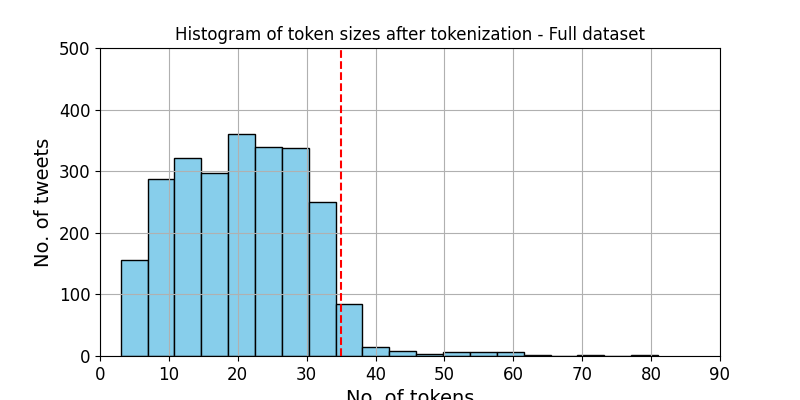
\includegraphics[width=\textwidth]{figures/token_pp_hist_vinai-bertweet-base.png}
        \caption{BERTweet}
        \label{fig: token_pp_hist_bertwteet}
    \end{subfigure}
    \begin{subfigure}[b]{0.48\textwidth}
        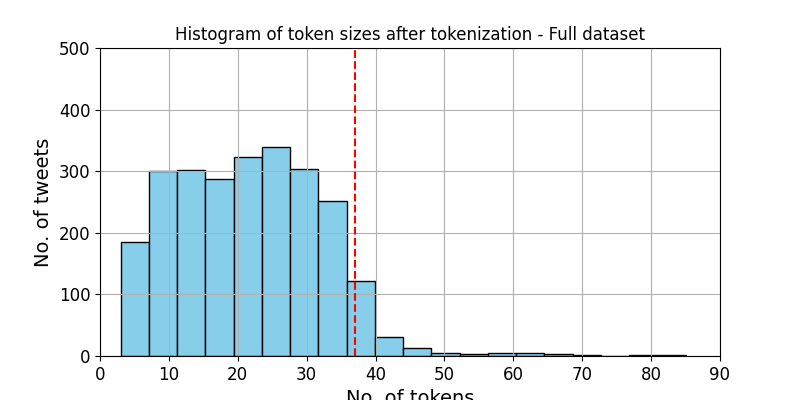
\includegraphics[width=\textwidth]{figures/token_pp_hist_prajjwal1-bert-tiny.png}
        \caption{BERT tiny}
        \label{fig: token_pp_hist_tiny}
    \end{subfigure}
    \hfill
    \begin{subfigure}[b]{0.48\textwidth}
        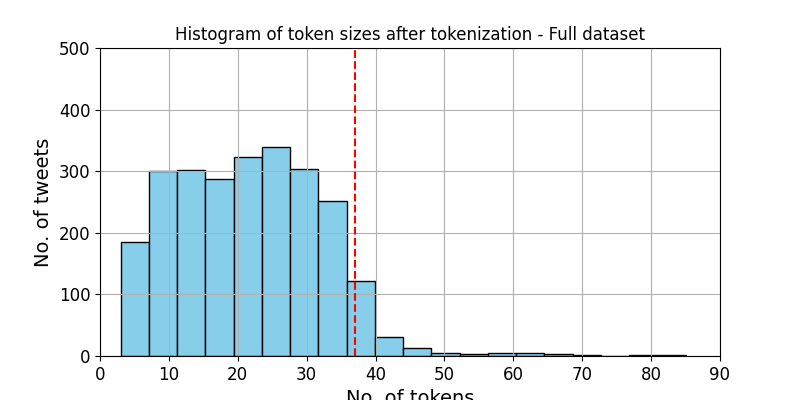
\includegraphics[width=\textwidth]{figures/token_pp_hist_distilbert-base-uncased.png}
        \caption{DistilBERT base uncased}
        \label{fig: token_pp_hist_distilbert}
    \end{subfigure}
    \begin{subfigure}[b]{0.48\textwidth}
        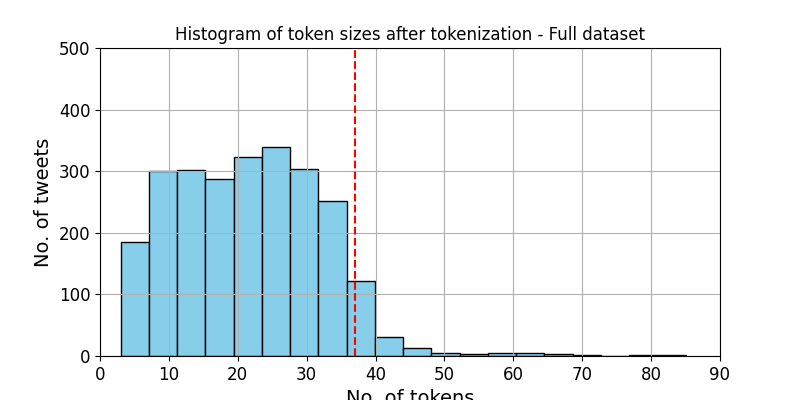
\includegraphics[width=\textwidth]{figures/token_pp_hist_google-mobilebert-uncased.png}
        \caption{MobileBERT uncased}
        \label{fig: token_pp_hist_mobile}
    \end{subfigure}
    \hfill
    \begin{subfigure}[b]{0.48\textwidth}
        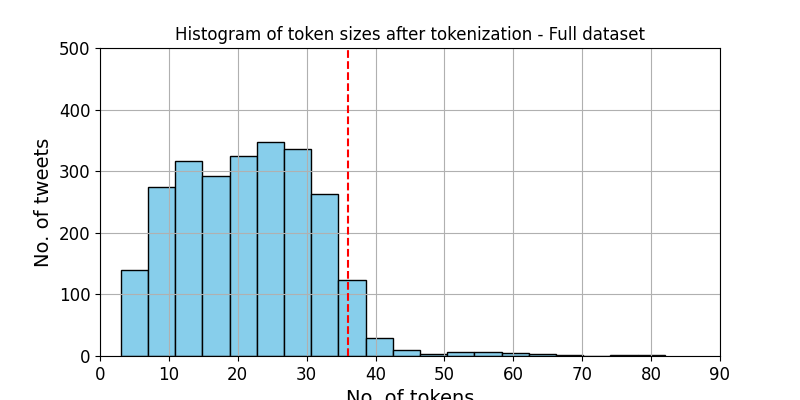
\includegraphics[width=\textwidth]{figures/token_pp_hist_roberta-base.png}
        \caption{Roberta base}
        \label{fig: token_pp_hist_roberta}
    \end{subfigure}
    \caption{The token count distribution for the full dataset of 3,449 tweets for all models.}
    \label{fig: apdxa_tokens}
\end{figure}